\section{Memoria FIFO (\texttt{fifo})}

La FIFO (First-In, First-Out) es el bloque que \textbf{desacopla} temporalmente los productores y consumidores de datos. En este proyecto se utilizan dos, como vimos en la figura~\ref{fig:uart-general}: una a la salida del receptor (\textbf{FIFO RX}) y otra a la entrada del transmisor (\textbf{FIFO TX}). Su función es absorber ráfagas y tolerar pequeñas desincronizaciones entre módulos.

\begin{figure}[H]
    \centering
    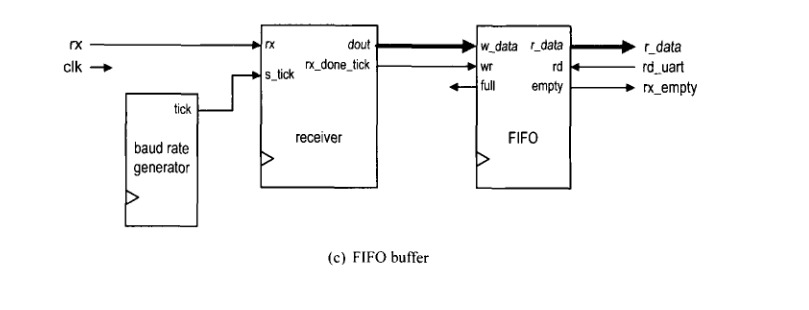
\includegraphics[width=0.78\textwidth]{img/FIFObuffer.jpeg}
    \caption{Inserción de una FIFO a la salida del receptor UART.}
    \label{fig:fifo-buffer}
\end{figure}

\subsection{Estructura y señales}
La FIFO es \textbf{sincronizada a un único reloj} (\texttt{clk}) y parametrizable:
\begin{itemize}
    \item \textbf{Ancho de palabra} \(W\) (bits por elemento).
    \item \textbf{Profundidad} \(N\) (cantidad de elementos).
\end{itemize}

Interfaz:
\begin{itemize}
    \item \texttt{w\_data} (entrada de datos), \texttt{wr} (pedido de escritura) y \texttt{full} (FIFO llena).
    \item \texttt{r\_data} (salida de datos), \texttt{rd} (pedido de lectura) y \texttt{empty} (FIFO vacía).
\end{itemize}

\subsection{Punteros y contador}
Internamente mantiene:
\begin{itemize}
    \item \textbf{Puntero de escritura} \(w\_ptr\) y \textbf{puntero de lectura} \(r\_ptr\), ambos de ancho \(\lceil \log_2 N \rceil\). Al incrementarse, \textbf{envolvieron} (wrap-around) de manera circular.
    \item \textbf{Contador de ocupación} \(count\) en el rango \(0 \ldots N\). De él se derivan las banderas:
    \[
        \texttt{empty} \Leftrightarrow count=0,\qquad
        \texttt{full}  \Leftrightarrow count=N.
    \]
\end{itemize}

\textbf{Nota de diseño:} si \(N\) \emph{no} es potencia de 2, conviene implementar un \emph{wrap} explícito (\(w\_ptr \leftarrow 0\) cuando \(w\_ptr=N-1\), idem \(r\_ptr\)) para garantizar que nunca se indexe fuera de \(0 \ldots N-1\).

\subsection{Escritura y lectura}
\paragraph{Escritura (lado productor).}
En el flanco ascendente de \texttt{clk}, si \texttt{wr} está activo y la FIFO \textbf{no} está llena, se copia \texttt{w\_data} en la posición indicada por \(w\_ptr\) y luego:
\[
w\_ptr \leftarrow w\_ptr + 1,\quad count \leftarrow count + 1.
\]

\paragraph{Lectura (lado consumidor).}
La salida \texttt{r\_data} refleja el contenido de la posición apuntada por \(r\_ptr\) (\emph{estilo FWFT, first-word fall-through}). Cuando el consumidor afirma \texttt{rd} y la FIFO \textbf{no} está vacía, en el próximo flanco:
\[
r\_ptr \leftarrow r\_ptr + 1,\quad count \leftarrow count - 1.
\]
Esto “avanza” la ventana y el siguiente dato queda disponible de inmediato en \texttt{r\_data} tras ese flanco.

\subsection{Lectura y escritura simultáneas}
Si en un mismo ciclo se cumple \(\texttt{wr}\wedge\neg\texttt{full}\) \emph{y} \(\texttt{rd}\wedge\neg\texttt{empty}\):
\[
w\_ptr \leftarrow w\_ptr + 1,\qquad r\_ptr \leftarrow r\_ptr + 1,\qquad count \text{ no cambia}.
\]
La ocupación permanece constante, lo que permite \textbf{canalizar} (pipeline) productor y consumidor sin bloqueo.

\subsection{Reset y mapeo en hardware}

Cuando se activa la señal de \texttt{reset}, la FIFO vuelve a su estado inicial:
\begin{itemize}
    \item Los punteros de lectura y escritura se ponen en cero.
    \item El contador de ocupación también se pone en cero.
\end{itemize}

Esto asegura que la memoria comience \textbf{vacía}.  

\subsection{Manejo correcto del \emph{handshake}}
\begin{itemize}
    \item El \textbf{productor} debe escribir solo cuando \(\neg\texttt{full}\).
    \item El \textbf{consumidor} debe leer solo cuando \(\neg\texttt{empty}\).
    \item Las banderas \texttt{full}/\texttt{empty} evitan \emph{overflow/underflow}.
\end{itemize}

\subsection*{Uso en el receptor (FIFO RX)}
A la salida del \texttt{uart\_rx}, cada vez que se completa una trama se genera \texttt{rx\_done\_tick}; ese pulso se utiliza como \texttt{wr} de la FIFO RX y el byte recibido ingresa como \texttt{w\_data}.  
El bloque \texttt{interface} actúa como \textbf{consumidor}: monitorea \texttt{empty}; cuando hay datos, aserta \texttt{rd} (señal \texttt{rd\_uart} en el diseño) para avanzar y tomar el próximo byte en \texttt{r\_data}. Así, el receptor puede seguir capturando tramas aunque el procesamiento sea más lento.

\subsection*{Uso en el transmisor (FIFO TX)}
La \texttt{interface} escribe en la FIFO TX el \textbf{resultado} de la ALU (\texttt{wr\_uart} como \texttt{wr}), siempre que \(\neg\texttt{full}\).  
El \texttt{uart\_tx} es el \textbf{consumidor}: cuando termina de enviar un byte, aserta \texttt{tx\_done\_tick} que hace de \texttt{rd} para tomar automáticamente el siguiente. En el \texttt{top}, la señal \texttt{tx\_start} se activa mientras la FIFO TX \textbf{no} esté vacía (\(\texttt{tx\_start} \leftarrow \neg \texttt{tx\_empty}\)), logrando una transmisión continua si hay datos en cola.
